% ---------------------------- README -----------------------------------------
% This file holds section three of the body of the Machine Intelligence I 
% script.
% -----------------------------------------------------------------------------

\newpage
\section{Probabilistic Methods I: Bayesian Inference}
\setcounter{equation}{0}

% -----------------------------------------------------------------------------
This chapter introduces a probabilistic approach to describe and
exploit the structure of stochastic relationships between multiple
variables. The general idea is to find a formally consistent
description of the world allowing to describe knowledge in terms of
``degrees of belief''. In this way, all knowledge can be stored in a
\emph{knowledge base} by assigning a degree of belief to each
\emph{atomic event}. Knowledge represented in this way can then be
exploited to \emph{infer} unobserved quantities, i.e.\ to reason about
the probability of making certain observations.

\subsection{Uncertainty and Inference}

% -----------------------------------------------------------------------------

\subsubsection{Degrees of Belief}
Knowledge can be stored in form of rules. Using deductive reasoning
and logic ($\rightarrow$ true or false) we can apply those rules to
observed data to infer further information beyond what is observed.
\begin{figure}[h] 
  \centering
\begin{tikzpicture}[font=\small\sffamily\bfseries,very thick,node distance = 4cm]
\node [frame] (rul) {rules};
\node [above=5mm] (kb) {knowledge base};
\node [above=0cm, left of=rul] (eve) {events};
\node [above=0cm, right of=rul] (pred)  {predictions};
\node [below=1.5cm] (comp)  {comparison};
\path [line] (eve) -> (rul);
\path [line] (rul) -> (pred);
\path [line] (eve) -> (comp);
\path [line] (pred) -> (comp);
\path [line] (comp) -> (rul);
\end{tikzpicture}
\end{figure}

\emph{But}: Does this really work in the real world?

\paragraph{Diagnosis example:} toothache (using first order logic)
\begin{enumerate}[(1)]
\item $\forall p$ $symptom(p, toothache) \Rightarrow disease(p,cavity)$ \\
\indent $\leadsto$ rule is wrong: not all patients with toothache have cavities (gum disease, abscess, $\ldots$)
\item $\forall p$ $symptom(p, toothache) \Rightarrow$ \\
 $disease(p, cavity) \lor disease(p, gum disease) \lor disease(p, abscess) \lor \ldots$ \\
$\leadsto$ almost unlimited list of possible causes
\item diagnostic rule to causal rule \\
 $\forall p$ $disease(p, cavity) \Rightarrow symptom(p, toothache)$ \\
$\leadsto$ rule is wrong: not all cavities cause pain
\end{enumerate}
$\Rightarrow$ First order logic fails in many situations! Examples:
\begin{itemize}
	\item complete set of antecedents and consequences too large
	\item no complete theory for the domain
	\item incomplete observations
	\item stochastic environments
\end{itemize}
$\Rightarrow$ How can we deal with the fact that we are almost never 100\% sure
about our rules?
\paragraph{Degrees of belief}\mbox{}\\
\emph{Proposition} $H$: Patient $p$ has a cavity.
\[ \begin{array}{ll}
	P(H): H \rightarrow [0,1] 
	& \text{assignment of numbers} \\\\
	P(H) = 0
	& H \text{ is false} \\\\
	P(H) = 1
	& H \text{ is true} \\\\
	0 < P(H) < 1
	& \text{quantifies our degree of belief}
\end{array} \]
\emph{Formal treatment:} Assume $P(H)$ to obey the laws of probability theory
\begin{itemize}
  \itl ''probabilities''
  \itl but: no justification via repeated observations and stochastic outcome
\end{itemize}
(for detailed treatment, see \cite{Jaynes2003})
\\\\
\emph{Application to Betting agents:} (de Finetti, 1931)
\\
''If agent 1 expresses a set of degrees of belief that violate the
axioms of probability theory, then there is a combination of bets by
agent 2 that guarantees that agent 1 will lose money all the time.''
\\\\
Example: \textcite[p.474]{RussellNorvig2003}\slideref{betting agents}

% -----------------------------------------------------------------------------

\subsubsection{The Description of the World}
We start with a "sufficiently complete" set of random variables to describe the state of the world. 

\paragraph{Random variables and propositions}
\begin{description}
\item[Random variable:] a ''part'' of the world whose ''status'' is initially unknown  $\leadsto X, Y, \ldots$
\item[Domain of a random variable:] ''values'' the variable can take on 
\indent $\leadsto x, y, \ldots$
\end{description}
\paragraph{Examples}\mbox{}\\
Boolean variables:\\
\indent variable: $cavity$; domain: $\{true, false\}$ \\
\indent proposition: $cavity = true$\\
Discrete ordinal variables:\\
\indent variable: $weather$; domain: $\{sunny, rainy, cloudy, snow\}$ \\
\indent proposition: $weather = sunny$ \\
Continuous variables: \\
\indent variable: $temperature$; domain: $\mathbb{R}_0^+$ \\
\indent proposition: $temperature \in [290K, 291K]$
\paragraph{Atomic events}\mbox{}\\
Description of the ''world'': complete set of random variables \\
\indent e.g. $cavity, \; toothache, \; weather$
\\\\
Atomic event: complete specification of the state of the world \\
\indent e.g. $cavity = true \land toothache = false \land weather = sunny$
\begin{itemize}
  \itl atomic events are mutually exclusive
  \itl set of atomic events must be exhaustive
  \itl proposition $\corresponds$ disjunction of atomic events
\end{itemize}
\indent $cavity = true$ is equivalent to: \\
\indent $(cavity = true \land toothache = false \land weather = sunny) \lor$ \\
\indent $(cavity = true \land toothache = true \land weather = rainy) \lor \ldots$ 

\paragraph{Prior (unconditional) probabilities}\mbox{}\\ 
Specification of one's knowledge about the world - in the absence of any other information \\
\indent e.g. $P(cavity=true) = 0.1$ \\
\indent\indent $P(cavity=true,toothache=false,weather=snow) = 0.02$
\\\\
Complete specification of domain knowledge: table of degrees of belief for all atomic events \\
\indent e.g. $P(cavity,toothache,weather)$

\paragraph{Conditional probabilities}\mbox{}\\
Specification of one's knowledge about the world - given a set of observations (the ''evidence'').
\[ \begin{array}{l}
	P(cavity = true | toothache = true) = 0.8 \\
	P( \underbrace{cavity = false}_{ \text{proposition} }
	| \underbrace{ toothache = true}_{\substack{\text{observation /} \\
						\text{evidence}}}
	) = 0.2
\end{array} \]
$\Rightarrow$ conditional probability
\begin{equation}
	P( \underbrace{C}_{\text{variable}} | \underbrace{t}_{\text{value}} 
		) = \frac{ \overbrace{P(C,t)}^{\substack{\text{joint} \\
						\text{probability}}} }{
				P(t)}
\end{equation}
\begin{equation} \tag{product rule}
	P(C,t) = P(C|t) P(t)
\end{equation}
$P(C|t)$: degree of belief in $C$, given \underline{all} we know is $t$.

% -----------------------------------------------------------------------------

\subsubsection{Probabilistic Inference Using Joint Probabilities}
\emph{Knowledge base:} $P(x,y,\ldots)$ degrees of belief for all atomic events
\\\\
What is the probability of a proposition given a set of observations?
\[ \begin{array}{lll}
	\text{query variable:}
	& X & \leftarrow \text{ probability of values to be inferred}\\\\
	\text{evidence variable:}
	& E_j & \leftarrow \text{ observed variables} \\\\
	\text{unobserved variables:} 
	& Y_j & \text{"hidden" or "nuisance" variables}
\end{array} \]
\begin{equation}
	P(x | \vec{e}) = \underbrace{ \frac{P(x, \vec{e})}{P(\vec{e})} }_{
		\substack{\text{def. of cond.} \\ \text{probability}}}
		= \underbrace{ \alpha P(x, \vec{e}) }_{\text{normalization}}
		= \underbrace{ \alpha \sum\limits_{\vec{y}} 
			P(x, \vec{e}, \vec{y}) }_{\text{marginalization}}
\end{equation}
$\frac{1}{\alpha} = P(\vec{e}) = \sum\limits_{x,\vec{y}} P(x,\vec{e},\vec{y})$ involves a
sum over many different combinations of $x$ and $\vec{y}$ which can be
costly to evaluate. However, this does not have to be computed explicitly, because:
\begin{equation}		\tag{normalization of probabilities}
	\sum\limits_x P(x|\vec{e}) \eqexcl 1 
\end{equation}
This only uses knowledge $P(x,\vec{e},\vec{y}$) stored in the
knowledge-base, the \emph{product rule} and normalization
(for an example, see \cite[pp. 475]{RussellNorvig2003}). \slideref{marginalisation}

\paragraph{Note:} If we have the complete probability table for all atomic events, we have all the relevant information to do inference. 
\paragraph{Problem:} this ansatz does not scale! Assume $N$ binary random
variables:
\begin{itemize}
	\itl table of joint probabilities has $2^N$ entries
	\itl summation over approx. $2^N$ entries for inference\\ 
		$N = 100 \leadsto 2^N \approx 1.3 \cdot 10^{30}$ 
		$\leadsto$ additional assertion needed
\end{itemize}

% -----------------------------------------------------------------------------

\subsubsection{Conditional Independence}
\begin{center} 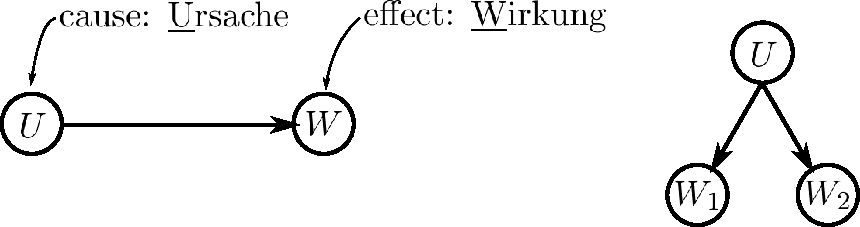
\includegraphics[height=2cm]{section3_fig2} \end{center}
Cause and effect: $P(W|U) \rightarrow$ ''causal rule''\\
One cause and two effects: $P(W_1, W_2|U) = P(W_1|U) P(W_2|U)$\\\\
\emph{Example: }$P(\text{toothache}, \text{catch}| \text{cavity})
	= P(\text{toothache}|\text{cavity})
		P(\text{catch}|\text{cavity})$

\paragraph{Definition of conditional independence}\mbox{}\\
Two random variables $X$ and $Y$ are conditionally independent given $Z$ if:
\begin{equation}
	P(X,Y|Z) = P(X|Z) P(Y|Z)
\end{equation}
and we write $X\perp Y |Z$.\\\\
\emph{Note:} Conditional independence is \underline{not} independence:\\
\indent $\Rightarrow$ $X$ and $Y$ are typically \underline{not}
independent.
\\\\
\emph{Note:} Conditional independence assertions are an important step
towards efficient inference algorithms: they enable a 
\emph{decomposition} of the knowledge base. To illustrate this fact,
consider a set of binary random variables: $w_1, w_2, \ldots, w_{N-1},
U$.
\\\\
Assuming conditional independence of effects given the cause:
\begin{equation}
	\underbrace{
		\underbrace{ P(w_1, w_2, \ldots, w_{N-1}, U) }_{
		2^N-1 \text{ table entries}}
		= \underbrace{ P(U) \prod\limits_{i = 1}^{N-1} P(w_i|U) }_{
		1 + 2(N-1) = 2N-1 \text{ table entries}} }_{
			\text{probabilities sum to one}}
\end{equation}
$\Rightarrow$ greatly reduces computational burden to determine joint distribution from $O\big(2^N\big)$ to $O(N):$ this would solve the scaling problem!
\\\\
This approach is called ``naive Bayes'' can even be useful in
situations where conditional independence does \emph{not} strictly hold.
\begin{center} 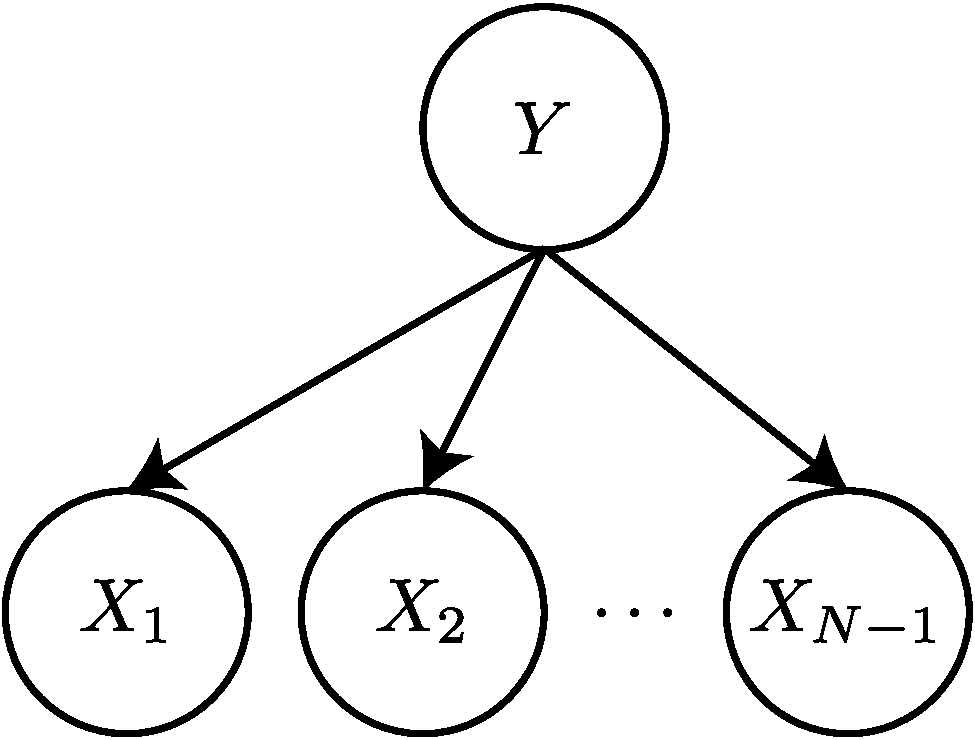
\includegraphics[height=2cm]{section3_fig3} \end{center}
$\Rightarrow$ use conditional probabilities as part of the model base
\subsubsection{Bayes' Theorem}
\paragraph{Common inference task:} Extract the causes underlying observations!
\[ \begin{array}{ll}
	\begin{array}{ll}
	\text{causal rule: } & P(W|U)P(U) \\\\
	\text{diagnostic rule: } & P(U|W)P(W) 
	\end{array}
	& \begin{array}{l}
	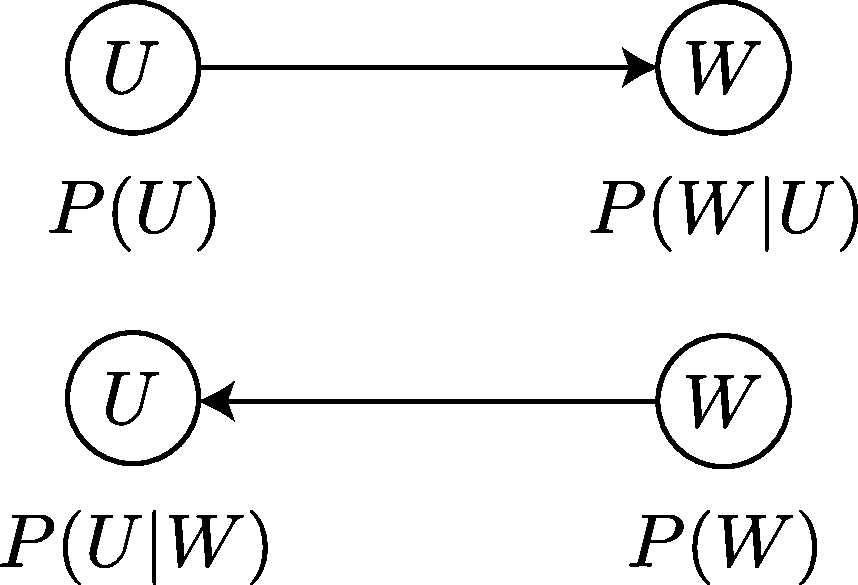
\includegraphics[height=1.5cm]{section3_fig4}
	\end{array}
\end{array} \]
\emph{Note:} In this graph, arrows do not represent causation but statistical dependency. 

\subsubsection*{Approach 1: causal knowledge base $\rightarrow$ diagnostic rule}
More generally, the joint probability $P(W,U)$ can be written as:
\begin{equation}\tag{Product rule}
	P(W|U)P(U) = P(W,U) = P(U|W)P(W)
\end{equation}
This can be used to infer $P(U|W)$ given $P(W|U)$ and $P(U)$ are known:
\begin{equation}\tag{Bayes' Theorem}
	P(U|W) = \frac{P(W|U)P(U)}{P(W)} = \alpha \; P(W|U)P(U)
\end{equation}
\underline{Comment 1:} Bayes' theorem holds for arbitrary random variables. ''Causes'' and ''effects'' were only used for illustration.

\subsubsection*{Approach 2: diagnostic knowledge base}
\emph{Advantage:} no calculations necessary to determine $P(U|W)$
\\\\
\underline{Comment 2:} Causal rules vs. diagnostic rules
\[ \left. \begin{array}{ll}
	\text{M:} & \text{meningitis} \\
	\text{S:} & \text{stiff neck}
\end{array} \right \} P(M|S) \]
Diagnostic knowledge base: $P(M|S)$ is directly stored. No computation
\\\\
causal knowledge base: $P(M|S) = \underbrace{ \alpha P(S|M) P(M) }_{
	\substack{\text{Bayes'} \\ \text{theorem}}}$\\
\indent $\rightarrow$ constructed from hospital records
\\\\
\emph{Problem:} Consider a sudden epidemic of meningitis: $P(M) \uparrow$ \\
\indent $\leadsto$ diagnostic knowledge base $p(M|S)$ cannot be updated easily

% -----------------------------------------------------------------------------

\newpage					% NEWPAGE for visual reasons
\subsection{Bayesian Networks}
\[ \text{Bayesian network} \left \{ \begin{array}{l}
	\text{- representation of the joint probability distribution} \\
	\text{- encoding of a collection of conditional independence statements}
\end{array} \right. \]
{\bf \underline{D}irected \underline{A}cyclic \underline{G}raphs (DAG)}
\begin{itemize}
	\item set of random variables 
		\begin{itemize}
			\itl nodes of the graph
		\end{itemize}
	\item direct influence between variables (e.g. causal relationships)
	\begin{itemize}
		\itl directed links between nodes
	\end{itemize}
	\item nodes are annotated with conditional probability distributions
		\[ P(x_i| parents(x_i)) \]
\end{itemize}
For details, see \textcite[ch. 14: Probabilistic Reasoning]{RussellNorvig2003}. 

\paragraph{Example:} Burglary detection in california: What is the probability of a burglary given that John and/or Mary call? 
\begin{center} \includegraphics[width=10cm]{section3_fig5} \end{center}
\begin{equation}
	P(J,M,A,B,E) = P(J|A)P(M|A)P(A|B,E)P(B)P(E)
\end{equation}
\emph{Bayesian network:}
\[ \begin{array}{lcl}
	\substack{\text{directed acyclic graph} \\ \text{annotated nodes}}
	& \longleftrightarrow &
	P(x_1, \ldots, x_N) = \prod\limits_{i=1}^n P(x_i|\mathrm{parents}(x_i))
\end{array} \]

\paragraph{Inference:} What is the probability of burglary - given that both Mary and John call?
\begin{center} 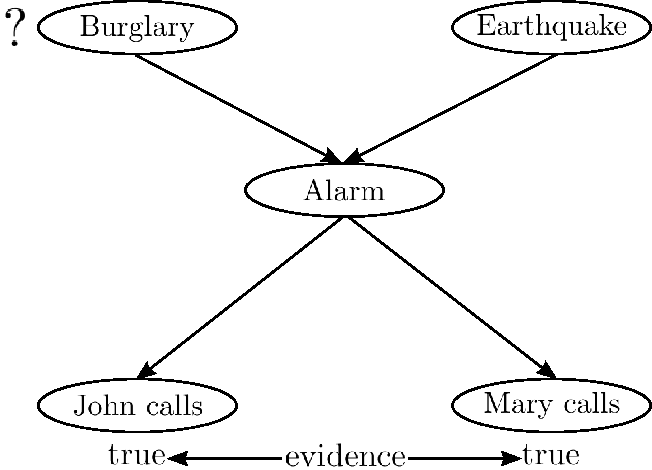
\includegraphics[width=8cm]{section3_fig6} \end{center}
To determine this probability, we need to marginalize over the two 
nuisance variables \texttt{Alarm} ($a$) and \texttt{Earthquake} ($e$):
\begin{equation}
	\begin{array}{lll}
	P(B|J=true, M=true) 
	& = & \underbrace{ \alpha P(B, J=true, M=true) }_{
		\substack{ \text{normalization} \\ \text{c.f. section 3.1.3}}} \\\\
	& = & \underbrace{ \alpha \sum\limits_{a,e} P(B, e, a, 
				J=true, M=true) }_{
		\text{marginalization}} \\\\
	& = & \alpha P(B) \sum\limits_e P(e) \sum\limits_a P(a|B,e) \\
	&& \cdot P(J=true|a) P(M=true|a) \\\\
	& = & \alpha \cdot \left \{ \begin{array}{ll}
			0.00059224 & \text{for } B=true \\\\
			0.0014919 & \text{for } B=false
		\end{array} \right.
	\end{array}
\end{equation}
Choose $\alpha$, such that sum is 1:
\begin{equation}
	P(B|J=true, M=true) = \left \{ \begin{array}{clc}
		0.284 & \text{for } B=true & 0.001 \\\\
		\underbrace{0.716}_{\substack{\text{evidence changed} \\
					\text{our assessment}}}
			& \text{for } B=false 
			& \underbrace{0.999}_{\text{Prior } P(B)}
	\end{array} \right.
\end{equation}
\textbf{Question:} How can we efficiently implement inference in larger and more complex Bayesian networks?

% -----------------------------------------------------------------------------

\subsubsection{Directed Acyclic Graphs}
Directed Acyclic Graphs (DAG's) provide useful graph structures to
represent probabilistic knowlege bases (cf.\ feedforward neural networks).
\begin{equation*}
\begin{array}{ll}
	\raisebox{-10mm}{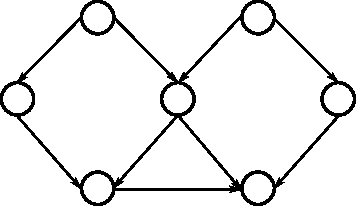
\includegraphics[width=4cm]{section3_fig7}}
	& \begin{array}{l}
		\text{Graph } G = (V, K) \\\\
		\begin{array}{ll}
			V & \rightarrow \text{ set of nodes} \\\\
			K & \rightarrow \text{ set of links}
		\end{array}
	\end{array}
\end{array}
\end{equation*}
\begin{description}
\item[path:]sequence $\big\{ x_i \big\}, i=1, \ldots, n$ of different nodes $x_i \in V$, such that $\big( x_i, x_{i+1} \big) \in K$ 
\item[cycle:] path with property  $x_1 = x_{n+1}$ 
\item[parents and children] of nodes:
\begin{center} \includegraphics[width=4cm]{section3_fig8} \end{center}
\end{description}
\textbf{DAGs and distributions:} Graphical models provide a link
between graph structures and probability distributions. This link
allows to use results from graph-theory to implement efficient
inference algorithms.\\\\
\textbf{Note:} Every DAG corresponds to a factorization of a joint PDF!
\begin{equation}
	\begin{array}{ccc}
	P(x_1, \ldots, x_n) & = & \prod\limits_{i=1}^n P(x_i|parents(x_i)) \\\\
	\text{''causal flow''} & \longleftrightarrow 
		& \text{well ordered nodes} \\\\
	\substack{\text{useful for construction} \\ \text{of compact networks}}
	&& \substack{\text{index of a node } x_i \text{ should always} \\
		\text{be larger than all indices of its parents}}
	\end{array}
\end{equation}

\paragraph{Topological sorting:} Naming nodes according to causal
flow. Application of \algfont{algorithm~\ref{alg:topological-sorting}} results
in a well ordered sorting of nodes corresponding to a factorization of
the joint pdf.
\begin{algorithm}
  \DontPrintSemicolon
  DAG with nodes without indices\;
  $i = 1$\;
  \While{nodes are left within DAG}{
    choose node without parents\;
    set index of node to $i$\;
    delete node and all its links from DAG\;
    $i\leftarrow i+1$\;
  }
\caption{Topological sorting}
\label{alg:topological-sorting}
\end{algorithm}

\paragraph{Comment:} conditional independence $\Rightarrow$ encoded by graph structure
\begin{enumerate}[(1)]
\item A node is conditionally independent of its non-descendants - given its parents
\item A node is conditionally independent of all other nodes in the network - given its parents, children and children's parents (Markov blanket)
\end{enumerate}
for further details, see \textcite[ch.14, Fig 14.4]{RussellNorvig2003}.\slideref{Markov Blanket}

\paragraph{Properties of DAGs}
\begin{itemize}
	\item efficient representation of knowledge about (causal) relationships 
		between variables
	\item \emph{topology}: qualitative relationships (causality, conditional 
		independence)
	\item \emph{annotation}: quantitative information (probability tables of pdfs)
	\item straightforward to construct
\end{itemize}
\emph{Problem}: DAGs do not provide an efficient representation for
inference (one of the central aims of using graphical models). Such a
respresentation, however, can be constructed on the basis of the
corresponding decomposable undirected graph.

% -----------------------------------------------------------------------------

\subsubsection{Decomposable Undirected Graphs}
\[\begin{array}{ll}
	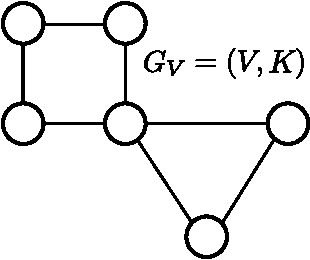
\includegraphics[width=4cm]{section3_fig9}
	& \substack{\text{undirected graph:} \\ 
		\text{graph with undirected links}}
\end{array} \]
\paragraph{Separator}\mbox{}\\
Consider $A, B, C \subset V$ (not necessarily disjoint)\\\\
$\Rightarrow C$ separates $A$ and $B$, if every path from an arbitrary node from $A (x_1 \in A)$ to an arbitrary node from $B (x_n \in B)$ passes through at least one node from $C$.
\[ \begin{array}{ll}
	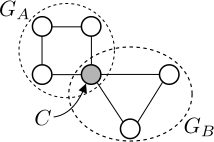
\includegraphics[width=4.5cm]{section3_fig10}
	& C \text{ separates } A \text{ and } B
      \end{array} \]
\textbf{Complete graph:} a graph in which every pair of nodes is connected by an edge.

\paragraph{Proper decomposition of $G = (V,K)$}\mbox{}\\
Consider $V = A \cup B \cup C$ with $A,B,C$ non-empty and disjoint
\\\\
$\Rightarrow A,B,C$ is a proper decomposition of $G$ if:
\begin{itemize}
	\itl $C$ separates $A$ and $B$
	\itl $C$ is complete 
\end{itemize}
\[ \begin{array}{ll}
	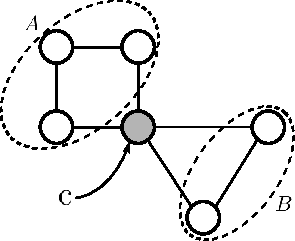
\includegraphics[width=4.5cm]{section3_fig11}
	& \substack{C \text{ separates } A \text{ and } B\\
		A,B,C \text{ is proper decomposition}}
\end{array} \]
\paragraph{Decomposable graph}
\begin{itemize}
	\itl complete graph \underline{or}
	\itl there exists a proper decomposition $A,B,C$ such that both 
		subgraphs $G_{A \cup C}$ and $G_{B \cup C}$ are both proper 
		decomposable
\end{itemize}
\[ \begin{array}{ccc}
	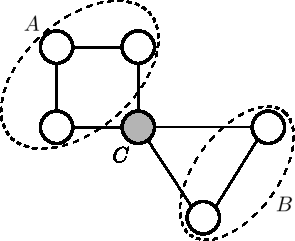
\includegraphics[width=4cm]{section3_fig12}
	& \includegraphics[width=4cm]{section3_fig13}
	& 
\includegraphics[width=4cm]{section3_fig14} \\\\
	\substack{ \text{not decomposable} \\
		\text{(no separator of } A \cup C \text{ is complete} \\
		\text{nor is } A \cup C \text{ complete)}}
	& \text{decomposable}
	& \text{decomposable or complete}
\end{array} \]
$\Rightarrow$ decomposition into \underline{maximally complete subgraphs (''cliques'')} separated by ''separators''

\begin{center} 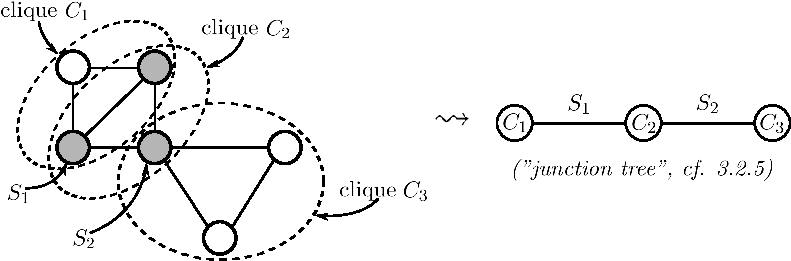
\includegraphics[width=12cm]{section3_fig15} \end{center}

\paragraph{Decomposable graphs and distributions: }
Decomposable graphs provide a useful factorization of the joint
distribution allowing to efficiently calculate marginals ($\rightarrow$
inference, see 3.2.4/5).


\begin{enumerate}[(1)]
\item $A$ is conditionally independent of $B$ given $C$ \\
$\Leftrightarrow A,B,C$ is a proper decomposition of $G$
\item $\begin{array}{ll}
	P(\vec{x}) = \frac{ \prod\limits_{\text{cliques }C} P_C(\vec{x}_C) }{
			\prod\limits_{\text{separators }S} P_S(\vec{x}_S)}
	& \substack{\text{decomposable graph} \\
		\longleftrightarrow \text{ factorization into} \\
			\text{marginal distributions}}
\end{array} $
\end{enumerate}
\textbf{Note:} The cliques (separators) are annotated by the marginal
probability distributions over the corresponding clique (separator)
variables.
\begin{center} \includegraphics[width=4cm]{section3_fig16} \end{center}
\begin{equation}\label{eq:marginalRepresentation}
	P(x_1, \ldots, x_6) = \frac{ \overbrace{ P(x_1, x_2, x_3) 
					P(x_2, x_3, x_4) P(x_4, x_5, x_6)}^{
						\text{cliques}}}{
				\underbrace{P(x_2, x_3)P(x_4)}_{
					\text{separators}}}
\end{equation}
This is a valid distribution, because:
\begin{eqnarray*}
\frac{ \prod_{C \in \mathcal{C}} P_C(\vec{x}_C) }{
			\prod_{S \in \mathcal{S}} P_S(\vec{x}_S)}
& = & \frac{ P(x_1, x_2, x_3) P(x_2, x_3, x_4) P(x_4, x_5, x_6)}{P(x_2, x_3)P(x_4)} \\
 & = &  P(x_1|x_2,x_3) P(x_2,x_3|x_4) P(x_4,x_5,x_6) \\
  & = & P(x_1|x_2,x_3) P(x_2|x_3,x_4) P(x_3) P(x_4|x_5,x_6) P(x_5|x_6) P(x_6) \\
  & = & \prod\limits_{i=1}^6 P(x_i|x_{i+1}, \ldots, x_6) \\
  & = & P(x_1, x_2, \ldots, x_6)
\end{eqnarray*}
\begin{center} 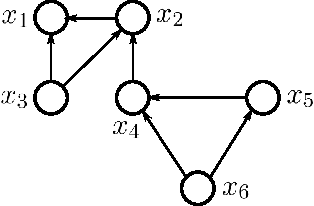
\includegraphics[width=4cm]{section3_fig17} \end{center}
\begin{itemize}
	\itr every decomposable undirected graph represents a valid probability 
		distribution
	\itr full marginalization: complexity $\mathcal{O}(2^n)$, $n$: cardinality of the 
		largest clique
\end{itemize}
\textbf{Note:} The general factorization into potentials is not unique!
\begin{equation}
	\begin{array}{ll}
		P(\vec{x}) \sim \frac{\prod\limits_{\text{cliques }C} 
					\psi_C (\vec{x}_C)}{
				\prod\limits_{\text{separators }S} 
					\psi_S (\vec{x}_S)} 

	\end{array}
\end{equation}
Shifting factors between terms in the numerator and denominator
results in the same value. This will become important for inference.
% -----------------------------------------------------------------------------

\newpage 						% --- for visual reasons
\subsubsection{Marginal Distributions and Inference on Decomposable Graphs}
The following example illustrates how the representation of the joint
distribution in terms of potential functions can be transformed into a
representation based on the marginal probabilities over the
corresponding cliques
(cmp.~\cite[p.~84]{CowellEtAl2003}). Consider the distribution
over 3 random variables $X,Y,Z$ described by the following graph:

\begin{center} 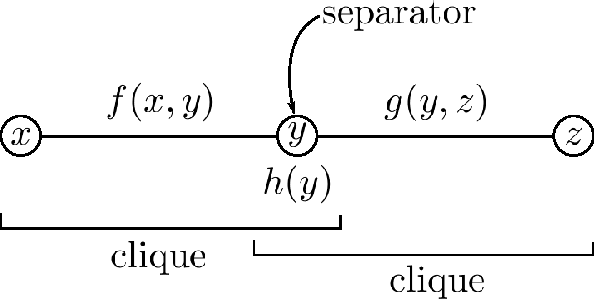
\includegraphics[width=8cm]{section3_fig18} \end{center}
\begin{equation}\label{eq:potentialRepresentation}
	P(x, y, z) = \alpha \frac{f(x, y) g(y, z)}{h(y)}
\end{equation}

\paragraph{Goal:} calculate factorization into marginals
\\
\emph{Starting point:} factorization into potentials (here: $f,g,h$) often straightforward to construct, e.g.
\begin{equation}
  P(x,y,z) = \frac{ \overbrace{P(x|y)}^{\corresponds f(x,y)}
    \overbrace{P(y|z)P(z)}^{\corresponds g(y,z)}}{
    \underbrace{1}_{\corresponds h(y)}}
\end{equation}
\begin{center} 
  
\includegraphics[width=6cm]{section3_fig19} 
\end{center}
Furthermore, inference problems lead to a potential-based representation for
the conditional probability distributions. \\\\
Consider, e.g.\ inference given observed evidence: $Z=z$
\begin{equation}
  P(x,y|z) = \frac{P(x,y,z)}{P(z)} = \alpha' P(x,y,z)
  = \alpha \frac{f(x,y) g(y,z)}{h(y)}
\end{equation}
indicator functions:
\begin{equation}
  E(z) = \left \{ \begin{array}{ll}
      1, & \text{if } Z = z\\
      0, & \text{else}
    \end{array} \right.
\end{equation}
\begin{equation}
  \underbrace{P(x,y|z)}_{P^{(z)}(X,Y,Z)} = 
  \alpha \frac{f(x,y)
    \overbrace{g(y,z)E(z)}^{\substack{
        \text{new clique} \\
        \text{- potential -}\\
        \text{after observing} \\
        \text{the evidence}}
    }}{h(y)}
\end{equation}
\begin{equation}
  \Rightarrow P^{(z)}(x, y, z) = \alpha
  \frac{f(x,y)g^{(z)}(y,z)}{
    h(y)}
\end{equation}

\paragraph{Calculation through message passing:}The representation of
the joint probability in terms of clique potentials
(eq.~\ref{eq:potentialRepresentation}) can be transformed into a
representation in terms of the marginal probabilities over the
corresponding cliques (cmp. \ref{eq:marginalRepresentation}) which is
useful e.g.\ to infer conditional probabilities.
\begin{enumerate}[(1)]
\item The marginal distribution of $P(x,y)$ can be calculated from the
  clique-representation
 \begin{equation}
	\begin{array}{ll}
		P(x,y) 
		& = \sum\limits_{z} P(x,y,z) \\\\
		& = \alpha \frac{f(x,y)}{h(y)} \underbrace{
			\sum\limits_{z} g(y,z)}_{\eqexcl h^*(y)} \\\\
		& = \alpha \underbrace{ f(x,y) \frac{h^*(y)}{h(y)} }_{
			\eqexcl f^*(x,y)}
	\end{array}
\end{equation}
This means that $f^*(x,y) \sim P(x,y)$ and can be calculated from the
potential $f(x,y)$ by passing to it a ``message'' containing the \emph{update ratio}
$\frac{h^*(y)}{h(y)}$ calculated from the clique potential $g(y,z)$
and the separator potential $h(y)$. This way we get a representation
of the joint distribution in terms of the updated (*) potentials: 
\begin{equation}
	\begin{array}{ll}
		P(x,y,z) 
		& = \alpha f(x,y) \frac{1}{h(y)} \frac{h^*(y)}{h^*(y)} 
			g(y,z)\\\\
		& = \alpha f^*(x,y) \frac{1}{h^*(y)}g(y,z)\\\\
	\end{array}
\end{equation}
\item The marginal distribution of clique $P(y,z)$ can be calculated in the same way
\begin{equation}
	\begin{array}{ll}
		P(y,z) 
		& = \sum\limits_x P(x,y,z) \\\\
		& = \alpha \underbrace{\bigg(\sum\limits_x f^*(x,y) \bigg)}_{
				\eqexcl h^+(y)} \frac{1}{h^*(y)} g(y,z)\\\\
		& = \alpha \underbrace{\frac{h^+(y)}{h^*(y)} g(y,z)}_{
				 \eqexcl g^+(y,z)}
	\end{array}
\end{equation}
Yielding the updated potential $g^+(y,z) \sim P(y,z)$ and the joint representation in terms of both updated potentials: 
\begin{equation}
	\begin{array}{ll}
		P(x,y,z) 
		& = \alpha f^*(x,y) \frac{h^+(y)}{h^+(y)}
			\frac{1}{h^*(y)} g(y,z)  \\\\
		& = \alpha f^*(x,y) \frac{1}{h^+(y)} g^+(y,z)
	\end{array}
\end{equation}
\item Marginal distribution of the separator $P(y)$
 \begin{equation}
	\begin{array}{ll}
		P(y) 
		& = \sum\limits_x P(x,y) \\\\
		& = \alpha \sum\limits_x f^*(x,y)\\\\
		& = \alpha h^+(y) \\\\
		& \Rightarrow h^+(y) \sim P(y)
	\end{array}
\end{equation}
\item Joint distribution: collecting terms shows that the updated representation is, indeed, based on the clique-marginal distributions. 
\begin{equation}
	\begin{array}{ll}
		P(x,y,z) 
		& = \alpha \frac{P(x,y)}{\alpha}
			\frac{\alpha}{P(y)} 
			\frac{P(y,z)}{\alpha}\\\\
		& = \frac{P(x,y)P(y,z)}{P(y)}
	\end{array}
\end{equation}
\end{enumerate}
\slideref{message passing\\ \& local\\ computation} 
\[ \text{message passing} \left \{ \begin{array}{l}
	\text{for calculating prior marginals} \\\\
	\text{for calculating posteriors marginals (after observation of 
		evidence)}
\end{array} \right. \]

% -----------------------------------------------------------------------------

\subsubsection{Belief Propagation and the Junction Tree Algorithm}
\paragraph{Overview}
\begin{enumerate}[(1)]
\item  \emph{definition of state variables \& construction of the Bayesian network:}
\begin{enumerate}[-a-]
	\item directed acyclic graph (expert analysis, causal relationship)
	\item topological sorting
	\item annotation with conditional probabilities (expert
          knowledge, extraction of fractions from database, ... inductive learning?)
        \end{enumerate}

\item \emph{ construction of the inference engine}
\[ \begin{array}{ccl}
	\text{-a-} & \text{directed acyclic graph} & \leftarrow \text{ annotated with 
					conditional pdfs} \\
	& \downarrow \\
	\text{-b-} & \text{moral graph}\\
	& \downarrow \\
	\text{-c-} 
& \text{undirected decomposable graphs} & \leftarrow \text{ annotated with
					clique and separator potentials}\\
	& \downarrow \\
	\text{-d-} & \text{junction tree} & \leftarrow \text{ final data structure for 
					message passing}
\end{array} \]

\item \emph{inference:} processing the evidence
\begin{enumerate}[-a-]	
  \item initialization
  \item modification of clique potentials by observed evidence (not when 
  just calculating prior)
  \item message passing (''belief propagation'')
  \item final marginalization within relevant clique
\end{enumerate}
\end{enumerate}


\paragraph{Details ad (2) -- Construction of the inference engine}\label{sec:details}
\begin{enumerate}[-a-]
\item directed acyclic graph
\item construction of the related moral graph \slideref{DAG\\$\downarrow$\\moral\\graph}
  \begin{itemize}
    \itr connect all parents of a node with undirected links (for 
    all nodes)
    \itr replace all directed links with undirected links 
  \end{itemize}
  \item construction of a related undirected decomposable graph\slideref{undirected\\ decompos.\\ graph} 
  \begin{itemize}
    \itr add undirected links such that all cycles of length four and
    larger contain a chord \itr chordal graph is always decomposable\footnote{for a proof, see Cowell et. al. theorem 4.4} \slideref{triangulation algorithm}
    \itr chordal graph is not unique 
    \itr construction of a chordal graph with cliques of minimal size is NP hard 
  \end{itemize}
  \item construction of a related junction tree
  \begin{itemize}
    \itr \emph{nodes of the junction tree}:\\
    maximal cliques of the decomposable graph
    \itr \emph{links of the junction tree}:\\
    connect neighboring maximal cliques annotated by the corresponding separators \slideref{construction of the junction tree}
    \itr after the first loop, the running intersection
    property holds, i.e. for all $1 < j \leq k$ 
    there exists one $i < j$, such that $C_j \cap
    \big( C_1 \cup \ldots \cup C_{i-1} \big) 
    \subseteq C_i$
    \itr but: nodes may not only be cliques, but could be 
    other complete subgraphs
    \itr second loop estimates those nodes
  \end{itemize}
\end{enumerate}

\paragraph{Details ad (3) -- Inference: processing of the evidence}
\label{sec:infer-proc-evid}
\begin{enumerate}[-a-]
  \item initialization of the clique and separator potentials   \slideref{initialization of cliques and separators}
  \begin{equation}	
    P(\vec{x}) = \prod\limits_k P(x_k|parents(x_k)) 
    \leftarrow \text{ from annotated DAG}
  \end{equation}
   \begin{algorithm}
     \DontPrintSemicolon
     Set all clique and separator potentials to $\psi_{C,S}(\vec{x}_{C,S}) = 1$\;
     \For{all nodes $x_k$ of the DAG}{
       Find a node of the junction tree which contains $x_k$ and its parents\; 
       Multiply corresponding clique potential with $P(x_k|parents(x_k))$}
     \caption{Initialization of clique potentials}
   \end{algorithm}

\item modification of clique potentials by observed evidence 
  \begin{itemize}
  \itr for given observations $\vec{X}_e = \vec{x}_e$, set clique potentials to:
  \begin{equation}
    P(\vec{x}/\vec{x}_e|\vec{x}_e) =
    \alpha P(\vec{x}) 
    \underbrace{\prod\limits_{j \in e}}_{
      \substack{\text{multiplied to} \\
        \text{the proposed} \\
        \text{clique potential}}}
    \underbrace{E(x_j)}_{\substack{\text{indicator
          functions}\\
        E(x_j) = \left\{ \begin{array}{ll}
            1, & \text{ if } X_j = x_j\\\\
            0, & \text{ else}
          \end{array} \right.}}
  \end{equation}
  \end{itemize}


  \item calculation of marginal probabilities: belief propagation
    \begin{itemize}
      \itr ''collect evidence'' (1st pass): choose a root node from the junction tree, broadcast ``request'' \& collect
      \[ \begin{array}{ll}
        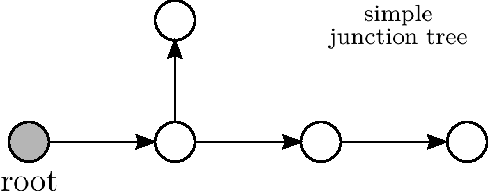
\includegraphics[width=4cm]{section3_fig20} 
        & \text{broadcast of request} \\\\
        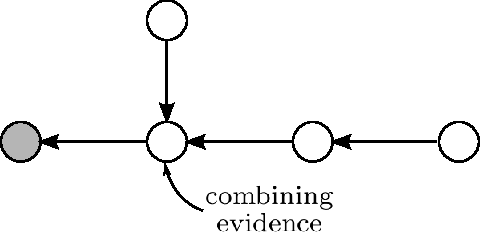
\includegraphics[width=4cm]{section3_fig21} 
      & \substack{ \text{transmission of 
          messages (and} \\
        \text{modification of 
          potentials)}}
    \end{array} \]
    \itr ''distribute evidence'' (2nd pass) 
    \[ \begin{array}{ll}
      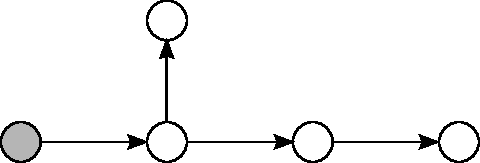
\includegraphics[width=4cm]{section3_fig22} 
      & \substack{ \text{transmission of 
          messages (and} \\
        \text{modification of 
          potentials)}}
    \end{array} \]
    \itR \begin{equation}
      \left. \begin{array}{l}
          P(\vec{x}) = \frac{\prod\limits_{\text{cliques }
              C} P_C(\vec{x}_C)}{\prod\limits_{
              \text{separators }S} P_S(
            \vec{x}_S)}
        \end{array} \right \} \text{marginal
        distributions}
    \end{equation}
  \end{itemize}
\item marginalization within relevant clique

\end{enumerate}

% -----------------------------------------------------------------------------

\newpage 						% --- for visual reasons
\subsection{Bayesian Inference and Neural Networks}

% -----------------------------------------------------------------------------
\subsubsection{Generative Models}
observations: $\vec{z}^{(\alpha)} = \big( \underbrace{ \vec{x}^{(\alpha)} }_{
	\substack{ \text{independent} \\ \text{variable} }}, 
	\underbrace{ \vec{y}_T^{(\alpha)} }_{ \substack{ \text{associated} \\
		\text{variable}} } \big), \alpha = 1, \ldots, p$
\\\\
true distribution:
\begin{equation}
	p_{(\vec{z})} = \underbrace{p_{(\vec{y} | \vec{x})}}_{
		\substack{ \text{conditional} \\ \text{probability} }}
	p_{(\vec{x})}
\end{equation}
\emph{previous approach:}
\begin{itemize}
	\itl construct a parametrized class $y_{(\vec{x};\vec{w})}$ of 
		(deterministic) predictors
	\itl inference is based on a single selected (optimal) predictor 
		$y_{(\vec{x}; \vec{w}^*)}$
\end{itemize}
\emph{generative model approach:}
\begin{itemize}
	\itl construct a parametrized class $p_{(\vec{y}|\vec{x};\vec{w})}$
		of (conditional) densities
	\itl inference is based on good ''generative models''
\end{itemize}
\begin{center}
$\underbrace{ \fbox{ \text{''generative'' model of a data source} } 
	}_{ \substack{
		\text{description of the data} \\
		\text{generation process} }}
\longrightarrow \fbox{ \text{observations} }$
\end{center}
\emph{Comment:}
\begin{itemize}
	\item[] models $p_{(\vec{z};\vec{w})}$ for unconditional densities
		$\leadsto$ unsupervised learning 
		\\ (e.g. ICA, mixture models)
	\item[] models $p_{(\vec{y}|\vec{x};\vec{w})}$ for conditional 
		densities $\leadsto$ supervised learning
\end{itemize}
\paragraph{Example I:} Generative model for simple regression
\begin{center}
\includegraphics[width=6cm]{section3_fig23} 
\end{center}
\emph{Description of the data generation process:}
\begin{equation}
  y_{(\vec{x})} = 
  \underbrace{ \widehat{y}_{(\vec{x};\vec{w})} }_{
    \substack{ 	\text{model of a deterministic} \\
      \text{relationship}}}
    + \underbrace{\widehat{\eta}}_{
      \substack{\text{model of the noise} \\
       \text{here: additive noise}}}
\end{equation}
The deterministic relationship is typically modeled with a
parametrized function e.g.\ a polynomial or a neural network. Noise is
often assumed to be additive but could also be multiplicative. Here, we model
noise with a parametrized distribution 
$\widehat{p}_{(\widehat{\eta}; \vec{\sigma})}$. 

\paragraph{Common noise models}\mbox{}\\
Additive Gaussian noise:
\begin{equation}
	\widehat{p}_{(y|\vec{x};\vec{w})} 
	= \frac{1}{\sqrt{2 \pi} \sigma} \exp \Bigg\{
		-\frac{ \big( y - \widehat{y}_{(\vec{x};\vec{w})} \big)^2 }{
			2 \sigma^2} \Bigg\}
\end{equation}
Additive Minkowski noise:
\begin{equation}
	\widehat{p}_{(y|\vec{x};\vec{w})} 
	= \frac{d \beta^{\frac{1}{d}}}{2 
		\underbrace{ \Gamma_{(\frac{1}{d})} }_{
			\substack{ 	\text{Gamma} \\
					\text{function} }
			} }
		\exp \Big\{ -\beta \big| y - \widehat{y}_{(\vec{x};\vec{w})}
			\big|^d \Big\}
\end{equation}
\indent $d = 1$: exponential function
\begin{equation}
	\widehat{p}_{(y|\vec{x};\vec{w})}
	= \frac{\beta}{2} \exp \Big\{ -\beta \big| y - 
		\widehat{y}_{(\vec{x};\vec{w})}	\big|^d \Big\}
\end{equation}
\indent $d = 2$: Gaussian distribution
\begin{center}
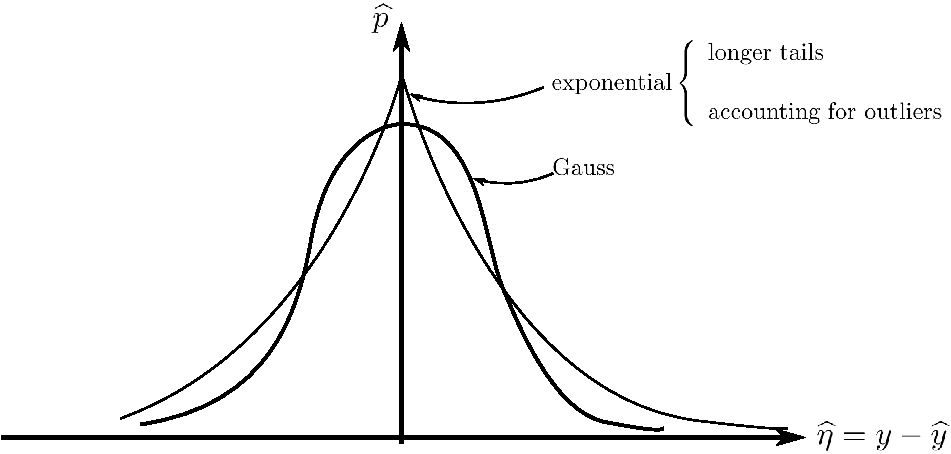
\includegraphics[width=12cm]{section3_fig24} 
\end{center}
\paragraph{Example II:} Classification for $c$ classes $C_k, k = 1, \ldots, c$
\\\\
\emph{Description of the data generation process:}
\begin{equation}
	p_{(C_k|\vec{x})} = y_{k(\vec{x})}
\end{equation}
\begin{itemize}
	\itl label noise (e.g. overlapping classes)
\end{itemize}
\emph{Model:}
\begin{equation}
	\widehat{p}_{(C_k|\vec{x};\vec{w})} = y_{k(\vec{x};\vec{w})}
\end{equation}
\begin{itemize}
	\itl general parametrized model (e.g. neural network: section 1.4.7)
\end{itemize}

% -----------------------------------------------------------------------------

\subsubsection{Bayesian Model Selection}
\emph{Reasoning under uncertainty} (cf.\ section 3.1.4)
\[ \begin{array}{lcl}
	\text{causal rules:}
	& \includegraphics[width=5cm]{section3_fig25} 
	& \text{''generative model''} \\\\
	\text{diagnostic rules:}
	& \includegraphics[width=5cm]{section3_fig26}
	& \substack{ 	\text{''model evaluation''} \\
			\leadsto \text{ evaluating the evidence}} \\\\
	& 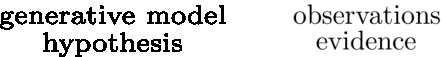
\includegraphics[width=5cm]{section3_fig27}
\end{array} \]
\emph{Degree of belief in a given model}
\begin{itemize}
	\itl set $\{ M_i \}$ of disjunct models (hypotheses) $M_i$
	\itl a random observed event $E$ (evidence)
\end{itemize}
\emph{Bayes rule:}
\begin{equation}
	\underbrace{ P_{(M_i|E)} }_{\substack{\text{posterior}}}
	= \frac{ \overbrace{ P_{(E|M_i)} }^{ \substack{ \text{likelihood}}}
	\overbrace{ P_{(M_i)} }^{\substack{\text{prior}}}
	}{ \underbrace{ P_{(E)} }_{\substack{\text{normalization constant}\\
		\text{(''evidence'')}}} }
\end{equation}
\textbf{Likelihood} $P_{(E|M_i)}$: probability of observing the evidence $E$, given that model $M_i$ is true $\Leftarrow \fbox{\text{''generative model''}}$
\\\\
\textbf{Prior} $P_{(M_i)}$: our degree of belief in $M_i$, before $E$ has been observed
\\\\
Initialization of prior beliefs $\rightarrow$ maximum entropy methods
\begin{equation}
	\begin{array}{lc}
	-\sum\limits_i P_{(M_i)} \ln P_{(M_i)} \eqexcl \max
	& \substack{ 	\text{find least informative} \\
			\text{prior beliefs}}
	\end{array}
\end{equation}
\emph{Constraints:}
\begin{equation}
	\begin{array}{lc}
	\sum\limits_i P_{(M_i)} = 1 
	& 
	\substack{	\text{normalization of} \\
			\text{probabilities}} \\\\
	\substack{ 	\text{information about (e.g.)} \\
			\text{moments of meanwhile} \\
			\text{quantities} }
	& \substack{ 	\text{formal description of} \\
			\text{prior knowledge}}
	\end{array}
\end{equation}
\begin{itemize}
	\itR solution using Lagrange multipliers
	\itR if no prior knowledge exists:
	\begin{equation}
		P_{(M_i)} = \mathrm{const.}
	\end{equation}
	\begin{equation}
		P_{(M_i|E)} \sim P_{(E|M_i)}
	\end{equation}
\end{itemize}

% -----------------------------------------------------------------------------

\subsubsection{Bayesian Prediction}
Predictions regarding future data $e$ will depend on both the observed
evidence $E$ and the model $M$ used. The \emph{predictive distribution} combines predictions from multiple models and weights them, depending on how probable these models are given the data observed so far ($\rightarrow$ posterior distribution of models/parameters given observed evidence).\\\\
\emph{The predictive distribution:}
\begin{equation}
	\substack{ 	\text{observations } E}
	\xrightarrow{ \substack{	\text{fundamental problem} \\
					\text{of prediction}} }
	\substack{	\text{degree of belief } P_{(e|E)} \\
			\text{into a new event } e}
\end{equation}
\begin{equation}
	\begin{array}{llc}
	P_{(e|E)} 
	& = \sum\limits_i P_{(e, M_i|E)}
	& \substack{ \text{marginalization} } \\\\
	& = \sum\limits_i P_{(e|M_i, E)} P_{(M_i|E)}
	& \substack{ \text{def. of conditional probability} } \\\\
	& \eqexcl \sum\limits_i P_{(e|M_i)} P_{(M_i|E)}
	& \substack{ \text{conditional independence assumption} }
	\end{array}
\end{equation}
\begin{itemize}
  \itr only ok if model fully describes data generation
  \itr only approximately fulfilled in reality
  \itR committee-ansatz (Bayesian committee)
\end{itemize}

\paragraph{Prediction and evaluation of distribution:}
After selection of a ''predicted attribute'' (see below) one can make a
decision based on $P_{(e|E)}$. In many cases it might not be
optimal to simply choose the maximally probable value because there are
additional constraints to consider, e.g. estimated loss if a
prediction error occurs. 
\\\\
\emph{Loss function:}
\begin{equation}
	C_{( \underbrace{ e }_{ \substack{	\text{true} \\
						\text{value}} }
		, \underbrace{ \widehat{e} }_{ \substack{
			\text{predicted} \\
			\text{value} \\
			\text{(based on } \\
			P_{(e|E)} \text{)}}} )}
\end{equation}
Instead of choosing the maximally probable value, it is therefore a common strategy to minimize the expected loss
\begin{equation}
	\widehat{e} = \argmin\limits_{\tilde{e}}
		\int d e C_{(e, \tilde{e})} P_{(e|E)}
\end{equation}

% -----------------------------------------------------------------------------

\subsubsection{Application: MLPs with weight decay}
For some simple models such as linear regression, the posterior
parameter distribution and the predictive distribution can be analysed
in closed form ($\leadsto$ Bayesian linear regression). For more
flexible models, exact analytical treatment is not available such that
evaluation of the predictive distribution requires approximation
techniques (e.g.\ sampling, variational inference). 

Here, we discuss another alternative, the \emph{Laplace
  approximation}, which (a) approximates the true posterior parameter
distribution with a Gaussian centered on a MAP estimate and (b)
assumes the network function to be approximately linear around this
point.

To determine the posterior parameter distribution from a given set of
training data we will (a) formulate the likelihood function for a
given class of generative models, (b) determine the maximum entropy
prior distribution, and (c) use Bayes rule to combine them.
\\

\emph{training data:} $\Big\{ \big( \vec{x}^{(\alpha)}, y_T^{(\alpha)} \big)
	\Big\}, \alpha = 1, \ldots, p$ \\

\emph{abbreviations:} $X = \Big\{ \vec{x}^{(\alpha)} \Big\}, 
	Y = \Big\{ \vec{y}_T^{(\alpha)} \Big\}$


\paragraph{(a) Construction of the model class}
$\rightarrow$ likelihood of the data 
\begin{equation}
	P_{\big( y_T^{(\alpha)}| \vec{x}^{(\alpha)}; \vec{w} \big)}
	\sim \exp \Big\{ -\beta \underbrace{ 
		e_{\big( y_T^{(\alpha)}, \vec{x}^{(\alpha)}; 
		\vec{w}\big)}^T }_{ \substack{
			\text{almost always possible,} \\
			\text{because } P \text{ positive}}}
	\Big\}
\end{equation}
\begin{equation}
	\begin{array}{ll}
	P_{(Y|\vec{x};\vec{w})}
	& \sim \prod\limits_{\alpha} \exp \Big\{ -\beta 
		e_{\big( y_T^{(\alpha)}, \vec{x}^{(\alpha)}; \vec{w}\big)}^T
		\Big\} \\\\
	& \sim \exp \Big\{ -\beta \sum\limits_{\alpha} 
		e_{\big( y_T^{(\alpha)}, \vec{x}^{(\alpha)}; \vec{w}\big)}^T
		\Big\} \\\\
	& \sim \exp \left\{-\beta E^T \right\}
	\end{array}
\label{eq:likelihoodData}
\end{equation}
where $E^T:=E_{(Y, \mathrm{x}; \vec{w})}$ denotes the training
error. This shows a direct relation between minimisation of the
mean squared error and Maximum likelihood estimation under the
assumption of additive Gaussian noise:
\begin{equation}
	P_{(Y| \vec{x};\vec{w})} = 
	\frac{1}{(2 \pi \sigma^2)^{\frac{p}{2}}} 
	\underbrace{
	\exp \Bigg\{ -\frac{1}{2 \sigma^2} 
		\overbrace{
		\underbrace{ \sum\limits_{\alpha = 1}^p }_{
			\substack{ \text{iid assumption}} }
		\Big( y_T^{(\alpha)} 
		- \underbrace{ \widehat{y}_{\big(\vec{x}^{(\alpha)}; \vec{w})}
			}_{\substack{ \rightarrow \text{ MLP}}}
		\Big)^2 }^{ \substack{ \text{''quadratic error''} } }
	\Bigg\}
	}_{ \substack{\text{additive Gaussian noise}}}
\end{equation}
\paragraph{(b) Construction of the prior:} Maximum entropy method
\begin{equation}
	-\sum\limits_{\vec{w}} P_{(\vec{w})} \ln P_{(\vec{w})} \eqexcl \max
\end{equation}
\begin{equation}
	\sum\limits_{\vec{w}} P_{(\vec{w})} = 1
\end{equation}
\begin{equation}
	\sum\limits_{\vec{w}} E_{(\vec{w})}^R P_{(\vec{w})} 
	= \underbrace{ E_0 }_{ \substack{	\text{prior} \\
						\text{knowledge}} }
\end{equation}
\emph{Solution using Lagrange multipliers:}
\begin{equation}
	- \sum\limits_{\vec{w}} P_{(\vec{w})} \ln P_{(\vec{w})} 
	+ \lambda \Bigg( \sum\limits_{\vec{w}} P_{(\vec{w})} - 1 \Bigg)
	- \alpha \Bigg( \sum\limits_{\vec{w}} E_{(\vec{w})}^R P_{(\vec{w})}
	- E_0 \Bigg) \eqexcl \max
\end{equation}
\begin{equation}
	\begin{array}{rcl}
	- \ln P_{(\vec{w})} - 1 + \lambda - \alpha E_{(\vec{w})}^R 
	& = & 0 \\\\
	\ln P_{(\vec{w})} & = & \lambda - 1 - \alpha E_{(\vec{w})}^R \\\\
	P_{(\vec{w})} & \sim & \exp \Big( -\alpha E_{(\vec{w})}^R \Big)
	\end{array}
\label{eq:priorParameters}
\end{equation}
$\lambda$ is found through normalization of prior probabilities
$\leftarrow$ equivalent to choosing a normalization factor
\\\\
$\alpha$: can be calculated - in principle - from the corresponding
constraint $\rightarrow$ often used as a hyperparameter
\\\\
\emph{Comment:} This gives the ``least informative'' prior
distribution $P(\vec{w})$ constraining the final solution as little as
possible. However, prior knowledge already explicitly put in
\begin{itemize}
	\itl choice of parametrization (i.e.\ model class)
	\itl choice of noise model
\end{itemize}

\paragraph{(c) Application of Bayes rule:}
making use of the distributions from eqs.~(\ref{eq:likelihoodData}) and (\ref{eq:priorParameters}), we get the posterior parameter distribution
\begin{equation}
	\begin{array}{ll}
	P_{(\vec{w}|Y, X)}
	& \sim P_{(Y|X; \vec{w})} P_{(\vec{w})} \\\\
	& \sim \exp \big\{ -\beta E^T - \alpha E^R \big\} \\\\
	& = \exp(-\beta R)
	\end{array}	
\end{equation}
\indent where:
\begin{equation}
	R = \underbrace{ p }_{ \sim \# \text{data} } E^T
	+ \underbrace{ \alpha^{'} }_{ \sim \# \text{hyperparameters} }
	E^R
\end{equation}
\begin{equation}
	\begin{array}{lc}
	\alpha^{'} = \frac{\alpha}{\beta} 
	& \substack{	\text{the more data points, the} \\
			\text{less important is the prior}}
	\end{array}
\end{equation}
\begin{itemize}
	\item formal equivalence to a regularized training error
	\item low $R \rightarrow$ high posterior
	\item noise model $\rightarrow$ form of training error
	\item prior knowledge $\rightarrow$ regularization term
\end{itemize}


\paragraph{Note:} The form of the posterior distribution gives a
probabilistic justification of the MLP with weight decay
\begin{equation}
	R = \frac{1}{2} \sum\limits_{\alpha = 1}^p \Big( y_T^{(\alpha)}
		- \widehat{y}_{(\vec{x}^{(\alpha)}; \vec{w})} \Big)^2
		+ \underbrace{ \frac{ \alpha }{2} \sum\limits_{k = 1}^{d} 
			\mathrm{w}_k^2 }_{ \substack{ \text{{\it 
			cf. section 1.4.6}}} }
\end{equation}
\emph{Comment:} Because for the MLP, $\hat{y}$ depends nonlinearly on
$\vec{w}$, this distribution is not simply a Gaussian and might have
multiple local optima.

% -----------------------------------------------------------------------------

\subsubsection{The ''maximum a posteriori'' method}
\emph{Prediction through Bayesian committee}:
\begin{equation}
	\begin{array}{lc}
	P_{(y|\vec{x};Y,X)} = \int P_{(y|\vec{x};\vec{w})}
		P_{(\vec{w}|Y,X)} d^d \vec{w}
	\end{array}
\end{equation}
\begin{itemize}
\item often no closed expression for the integral
\item due to large number of model parameters, numerical methods to
  approximate high dimensional integrals (e.g.\ MCMC, variational
  Bayes) are often either time-consuming or inaccurate
\item MAP method provides an efficient \emph{approximation}
\end{itemize}
(see also \textcite[ch. 5.7]{Bishop2006})

\paragraph{The MAP-assumption:} Posterior has a localized maximum
\begin{center}
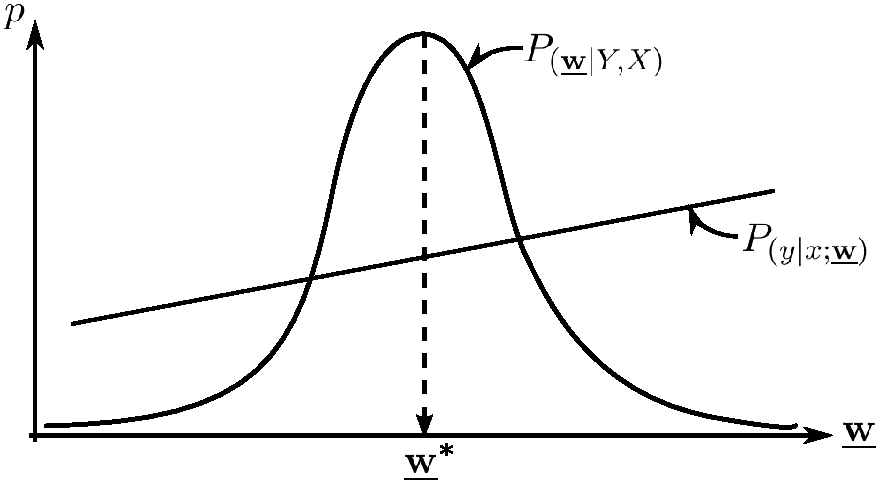
\includegraphics[width=8cm]{section3_fig28} 
\end{center}
\begin{equation}
	\begin{array}{lll}
	\vec{w}^* 
	& = \argmax\limits_{\vec{w}} P_{(\vec{w}|Y, X)} \\\\
	& = \argmin\limits_{\vec{w}} \underbrace{
		\big(p E^T + \alpha^{'} E^R \big) }_{ R }
		& \leftarrow \text{''MAP solution''}
	\end{array}
\end{equation}
We will use this assumption to approximate the \emph{predictive
  distribution}
\begin{equation}
	P_{(y|\vec{x};Y,X)} \sim \int \underbrace{
		\exp \big( -\beta e_{(y,x;\vec{w})}^T \big) }_{
			\substack{ \text{individual} \\ \text{likelihood} }}
		\underbrace{ \exp \big( -\beta R_{(\vec{w}, Y, X)} \big) }_{
			\substack{ \text{posterior} } }
		d^d \vec{w}
\end{equation}
This can be a good approximation e.g.\ when the posterior is highly
concentrated around $\vec{w}^*$. The approach used here involves two
approximations around the mode $\vec{w}^*$:

\paragraph{(1) Gaussian approximation of the posterior around $\vec{w}^*$:}
(Taylor expansion to $2^\mathrm{nd}$ order at
$\vec{w}^*$).\footnote{As the expansion is around the maximum
  $\vec{w}^*$, first order terms vanish here.}
\begin{equation}
	R_{(\vec{w}, Y, X)} = R_{(\vec{w}^*, Y, X)} + \frac{1}{2} 
		\sum\limits_{i,j} (\mathrm{w}_i - \mathrm{w}_i^*)
		\underbrace{ \frac{\partial^2 R}{\partial \mathrm{w}_i
			\partial \mathrm{w}_j} }_{
				\substack{ H_{ij} \text{: Hesse matrix}} }
		\bigg|_{\vec{w}^*} (\mathrm{w}_j - \mathrm{w}_j^*)
\end{equation}
\paragraph{(2) Linear approximation of the individual likelihood:}
Taylor expansion of the models input-output function around
$\vec{w}^*$ to $1^{\mathrm{st}}$ order
\begin{equation}
	e_{(y,\vec{x};\vec{w})}^T = e_{(y,x;\vec{w}^*)}^T 
	+ \sum\limits_i \frac{\partial e^T}{\partial \mathrm{w}_i} 
	\bigg|_{\vec{w}^*} (\mathrm{w}_i - \mathrm{w}_i^*)
\end{equation}
Result of the integration ({\it calculation see supplementary material})
\begin{equation}\label{eqn:predictiveDistributionAGN}
	P_{(y|\vec{x};Y,X)} \sim \exp \Bigg\{
		\underbrace{ -\beta e^T }_{ \substack{
			\text{individual} \\
			\text{likelihood} \\
			\text{for the MAP} \\
			\text{''model''} \vec{w}^*}}
		+ \frac{\beta}{2} \bigg( \underbrace{ 
			\frac{\partial e^T}{\partial \vec{w}} }_{
			\substack{ 	\text{correction for} \\
					\text{uncertainty} \\
					\text{(}2^{\mathrm{nd}}
					\text{ order)} \\
					\text{in estimating} \\
					\text{the model} \vec{w} }} \bigg)
		\vec{H}^{-1} \frac{\partial e^T}{\partial \vec{w}} \Bigg\}
		\Bigg|_{\vec{w}^*}
\end{equation}
For the MLP with additive Gaussian noise and weight decay, the corresponding terms are:
\begin{equation*}
	\beta = \frac{1}{\sigma^2}
%\end{equation}
\qquad \quad
%\begin{equation}
	e_{(\vec{x},y;\vec{w})}^T = \frac{1}{2} \big( y - 
		\underbrace{ \widehat{y}_{(\vec{x};\vec{w})} }_{ 
			\substack{ \text{MLP}}}
		\big)^2
%\end{equation}
\qquad \quad
%\begin{equation}
	\frac{\partial e^T}{\partial \vec{w}} = -\big( y - 
		\widehat{y}_{(\vec{x};\vec{w})} \big) 
	\underbrace{ \frac{\partial \widehat{y}}{\partial \vec{w}} }_{
		\eqexcl \vec{g}}
\end{equation*}
inserting into (\ref{eqn:predictiveDistributionAGN}) yields
\begin{equation}
	P_{(y|\vec{x};Y,X)} \sim \exp \bigg\{ -\frac{1}{2\sigma^2} 
	\big( \underbrace{ 1 }_{\substack{ \text{noise} \\ \text{model}}}
	- \underbrace{ \vec{g}^T \vec{H}^{-1} \vec{g} }_{
		\substack{	\text{correction for} \\
				\text{uncertainty in the} \\
				\text{determination of} \\
				\text{model parameters}} }
	\big) \Big|_{\vec{w}^*} \big( y - \widehat{y}_{(\vec{x}; \vec{w}^*)}
	\big)^2 \bigg\}
\end{equation}
This is a Gaussian centered on the model prediction ($M_{\vec{w}^*}$) whose
variance depends on the width of the posterior ($\rightarrow$ noise
model):
\begin{equation}
  \sigma_y^2 \eqexcl \frac{\sigma^2}{1 - \vec{g}^T \vec{H}^{-1} \vec{g}} \Big|_{\vec{w}^*}
\end{equation}
width of posterior $\uparrow \leadsto$ ''$\vec{H}^{-1} \uparrow$''
$\leadsto (1 - \vec{g}^T \vec{H}^{-1} \vec{g}) \downarrow \leadsto
\sigma_y^2 \uparrow$ \slideref{MacKay(1992)\\Fig.4b}.\\\\
For a more detailed discussion of the theoretical approach, see \textcite{MacKay1992c}.

\paragraph{Comments} 
\begin{enumerate}[(1)]
\item $\vec{w}^*$ is referred to as the ''MAP-solution'' \\
\begin{equation}
	\vec{w}^* = \argmin\limits_{\vec{w}} \big( p E^T + \alpha^{'} E^R \big)
\end{equation}
Formal equivalence between MAP solution and regularized ERM:
\begin{equation}
	E^T  \corresponds- \log \mathrm{likelihood} \qquad \qquad
	E^R  \corresponds - \log \mathrm{prior}
\end{equation}
\item \emph{Efficient calculation of the relevant terms for MLPs}\\
  $\vec{g}$ can be calculated via backpropagation, for calculation of
  $\vec{H}^{-1}$, see e.g.\ \textcite[ch.\ 5.4]{Bishop2006}.
\item $P_{(y|\vec{x};Y,X)} \sim \exp (-\beta e^T) \big|_{\vec{w}^*}$
  is sometimes referred to as the \emph{MAP solution} for the output
  distribution

\item The solution illustrates \emph{2 types of uncertainty:} 
  \begin{itemize}
  \item uncertainty inherent in the generating process ($\rightarrow \sigma^2$)
  \item precision of estimated model ($\rightarrow 1 - \vec{g}^T \vec{H}^{-1} \vec{g}$)
  \end{itemize}
\end{enumerate}
% -----------------------------------------------------------------------------

\subsubsection{Prediction of attributes (point prediction)}
\emph{Loss-function:} $C_{(y, \widehat{y})}$, real valued attributes
\\\\
\emph{Minimization of expected loss:}
\begin{equation}
	\widehat{y}_{(\vec{x})} = \argmin\limits_{\tilde{y}}
	\int dy C_{(y, \tilde{y})} P_{(y|x;Y,X)}
\end{equation}
\begin{center}
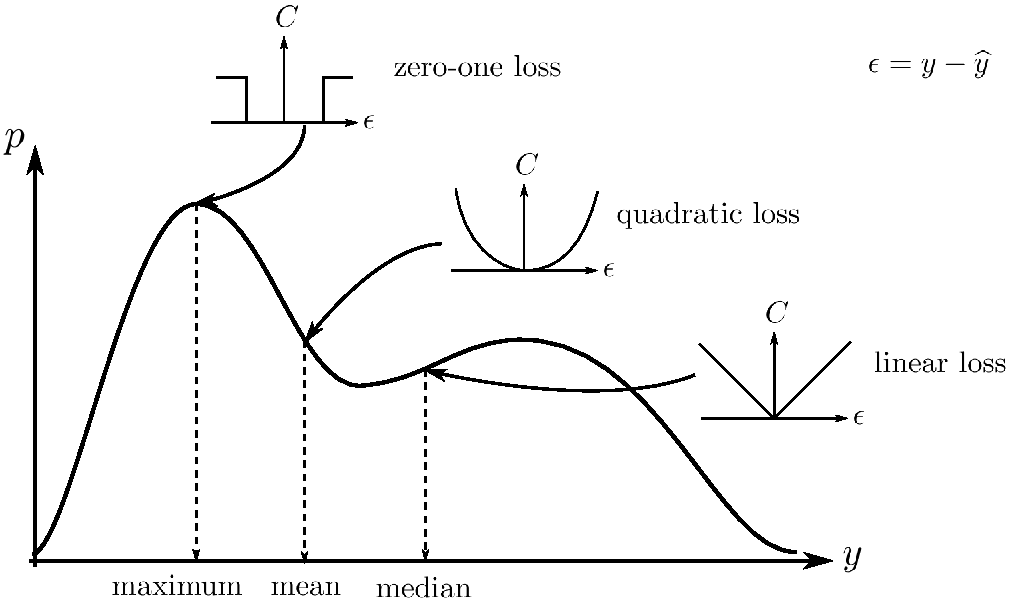
\includegraphics[width=12cm]{section3_fig29} 
\end{center}
For the Gaussian density: maximum $\corresponds$ mean $\corresponds$ median\\
$\Rightarrow$ predictions coincide

\paragraph{Example:} MLP with weight-decay, Gaussian approximation (MAP)
\begin{equation}
	\begin{array}{ll}
	\vec{w}^*
	& = \argmin\limits_{\vec{w}} \big( p E^T + \alpha^{'} E^R \big) \\\\
	& = \argmin\limits_{\vec{w}} \bigg\{ \frac{1}{2} 
		\sum\limits_{\alpha = 1}^p \Big( y_T^{(\alpha)} - 
		\widehat{y}_{\big( \vec{x}^{(\alpha)}; \vec{w} \big)}
		\Big)^2 + \frac{\alpha^{'}}{2} \sum\limits_{k = 1}^d
		\mathrm{w}_k^2 \bigg\}
	\end{array}
\end{equation}
predictor: ''optimal'' network: $\widehat{y}_{(\vec{x};\vec{w}^*)}$

% -----------------------------------------------------------------------------
